% Material found at https://www.elsevier.com/authors/author-schemas/latex-instructions

\documentclass{elsarticle}

\usepackage{lineno,hyperref}
\modulolinenumbers[5]

%=== Added for MU paper ====
\usepackage{color,soul} %% this was needed to have highlighted text
\usepackage{graphicx}
\usepackage{hyperref}
\usepackage{amsmath}
\usepackage{mathtools}
\usepackage{nomencl}
\makenomenclature
\graphicspath{{./figures/}}

\journal{Reliability Engineering \& System Safety}

%%%%%%%%%%%%%%%%%%%%%%%
%% Elsevier bibliography styles
%%%%%%%%%%%%%%%%%%%%%%%
%% To change the style, put a % in front of the second line of the current style and
%% remove the % from the second line of the style you would like to use.
%%%%%%%%%%%%%%%%%%%%%%%

%% Numbered
\bibliographystyle{model1-num-names}

%% Numbered without titles
%\bibliographystyle{model1a-num-names}

%% Harvard
%\bibliographystyle{model2-names.bst}\biboptions{authoryear}

%% Vancouver numbered
%\usepackage{numcompress}\bibliographystyle{model3-num-names}

%% Vancouver name/year
%\usepackage{numcompress}\bibliographystyle{model4-names}\biboptions{authoryear}

%% APA style
%\bibliographystyle{model5-names}\biboptions{authoryear}

%% AMA style
%\usepackage{numcompress}\bibliographystyle{model6-num-names}

%% `Elsevier LaTeX' style
%\bibliographystyle{elsarticle-num}
%%%%%%%%%%%%%%%%%%%%%%%

\begin{document}

\begin{frontmatter}

\title{Multi-Unit PRA: a Simulation-Based Approach}
%% \tnotetext[mytitlenote]{Fully documented templates are available in the elsarticle package on \href{http://www.ctan.org/tex-archive/macros/latex/contrib/elsarticle}{CTAN}.}

%% Group authors per affiliation:
\author{D. Mandelli, C. Parisi, A. Alfonsi, D. Maljovec, S. St Germain, R. Boring, S. Ewing, C. Smith}
\address{Idaho National Laboratory (INL), 2525 Fremont Ave, 83402 Idaho Falls (ID), USA}

\author{M. Rasmussen}
\address{Norwegian University of Science and Technology (NTNU)}

\begin{abstract}
  Risk importance measures are indexes that are used to rank systems, 
structures and components (SSCs) using risk-informed methods. 
The most used/known measures are: Risk Reduction Worth (RRW), 
Risk Achievement Worth (RAW), Birnbaum (B) and Fussell-Vesely (FV). 
Once obtained from classical Probabilistic Risk Analysis (PRA) analyses, 
these risk measures can be effectively employed to relatively rank
component importance.
In contrast to classical PRA methods, 
Dynamic PRA methods couple stochastic models with safety analysis 
codes to determine risk associate to complex systems such as nuclear 
plants. Compared to classical PRA methods, simulation-based approaches
can evaluate with 
higher resolution the safety impact of timing and sequencing of events 
on the accident progression. 
The objective of this paper is to present a series of methods that 
can be employed to measure risk importance of components which are 
part of complex systems such as nuclear power plants.
The first set of measures are directly derived from classical risk 
importance measures (e.g., RRW, RAW, B and FV) and that can be employed
to any Dynamic PRA analysis.
In addition, we provide a set of risk importance measures that capture the 
dynamic nature of the problem and provide insight related to plant safety 
margins.

\end{abstract}

\begin{keyword}
%% keywords here, in the form: keyword \sep keyword
Multi-unit \sep PRA \sep Dynamic PRA \sep Reduced Order Modeling \sep Surrogate Model
\end{keyword}

\end{frontmatter}

\linenumbers

\printnomenclature[1in]

\nomenclature{LWRS}{Light Water Reactor Sustainability}
\nomenclature{PWR}{Pressurized Water Reactor}
\nomenclature{RAVEN}{Risk Analysis Virtual ENvironment}
\nomenclature{ROM}{Reduced Order Model}
\nomenclature{SFP}{Spent Fuel Pool}
\nomenclature{ROM}{Reduced Order Modeling}
\nomenclature{RISMC}{Risk Informed Safety Margin Characterization}	

\section{Introduction}
\label{sec:introduction}
RAVEN (\textbf{R}isk \textbf{A}nalysis \textbf{V}irtual \textbf{EN}vironment)~\cite{Nureg1150}  is one of the many INL-developed software tools researchers can 
use to identify and 
increase the safety margin in complex systems (e.g. Nuclear Power Plants). It is a modular or ``plug-able'' framework that can be coupled with other computer 
modeling systems. RAVEN is capable to agnostically communicate with any system 
code. This agnosticism includes providing Application Programming Interfaces (APIs). These APIs are used to allow RAVEN to interact with any code as long as all 
the parameters that need to be perturbed are accessible through input files or via python interfaces. 
As a generic software framework, RAVEN is designed to perform parametric and probabilistic analysis based on the response of complex system codes. RAVEN is 
capable of investigating the system response as well as the input space using standard sampling techniques (e.g Monte Carlo, Grid, or Latin Hyper Cube), but its 
strength is focused toward system feature discovery, such as limit surfaces (i.e. separating regions of the input space leading to system failure, using dynamic 
supervised learning techniques), and advanced data analysis methodologies (i.e. Topology-based domain decomposition, Data Mining, Clustering, etc.).

The development of RAVEN has begun in 2012 to satisfy the need to provide a modern risk evaluation framework. RAVEN principal assignment is to provide the 
necessary software and algorithms in order to employ the concept developed by the Risk Informed Safety Margin Characterization (RISMC) path-
way~\cite{RISMC}. 
RISMC is one of the pathways defined within the Light Water Reactor Sustainability (LWRS) program. In the RISMC approach, the goal is not just specifically 
identifying the frequency of an event potentially leading to a system failure, but also to analyze the ``distance'' and the drivers toward the happening of key 
safety-related events. This approach may be used in identifying and increasing the safety margins related to those events. A safety margin is a numerical value 
quantifying the probability that a safety metric (e.g. as peak pressure in a pipe) is exceeded under certain conditions. The initial development of RAVEN has 
been focused on providing dynamic risk assessment capability to RELAP-7~\cite{RELAP7}, currently under development at the INL. All the methodologies
developed have been modularized in order to be applied to any computer modeling system (e.g., BISON, RELAP-7, RELAP5-3D, MELCOR, etc.).

The aim of this manuscript is to present a peculiar capability within the RAVEN framework named \textit{``EnsembleModels''}.

RAVEN is currently able to construct multi-targets Reduced Order Models (Ref.4), which are aimed to represent the response of a system (in a 
fixed configuration) for multiple Figures of Merits (FOMs) and time-dependent ROMs (see Ref.5). These capabilities represent the initial steps for a larger 
implementation about the interaction of multiple models. In fact, in several cases, multiple models need to interface with each other since the initial conditions of 
one are dependent on the outcomes of another.
To better understand the problem that here is solved, it is useful to consider two simple examples:
\begin{enumerate}
  \item The following problem is considered: a weather forecast simulation code ``a'' is used to compute the external (i.e. ambient) temperature in a certain location. 
  A second model ``b'' is inquired to compute the average temperature in a room having as boundary condition, among several others, the external ambient 
  temperature. The response of the model ``b'' depends on the outcome of the model ``a'';
   \item Two different simulation codes are considered: a) a code that is meant to compute the thermal conductivity of the ceramic Uranium Dioxide (UO2) as 
   function of the Temperature, and b) a Thermal-hydraulic (TH) code that is used to compute the Temperature field of a reactor, whose heat conduction depends on 
   the thermal conductivity value. As easily inferable, the two models are mutual dependent, determining in a non-linear system of equations.
\end{enumerate}
The two reported examples are only aimed to illustrate the reason why the creation of a framework to make interact different models is a key development for the 
advancement of RAVEN as a comprehensive calculation flow driver. Before reporting how the ensemble-models have been implemented, it is necessary to briefly 
describe the representative Model ``entities'' that are available in RAVEN.



\begin{figure}
    \centering
    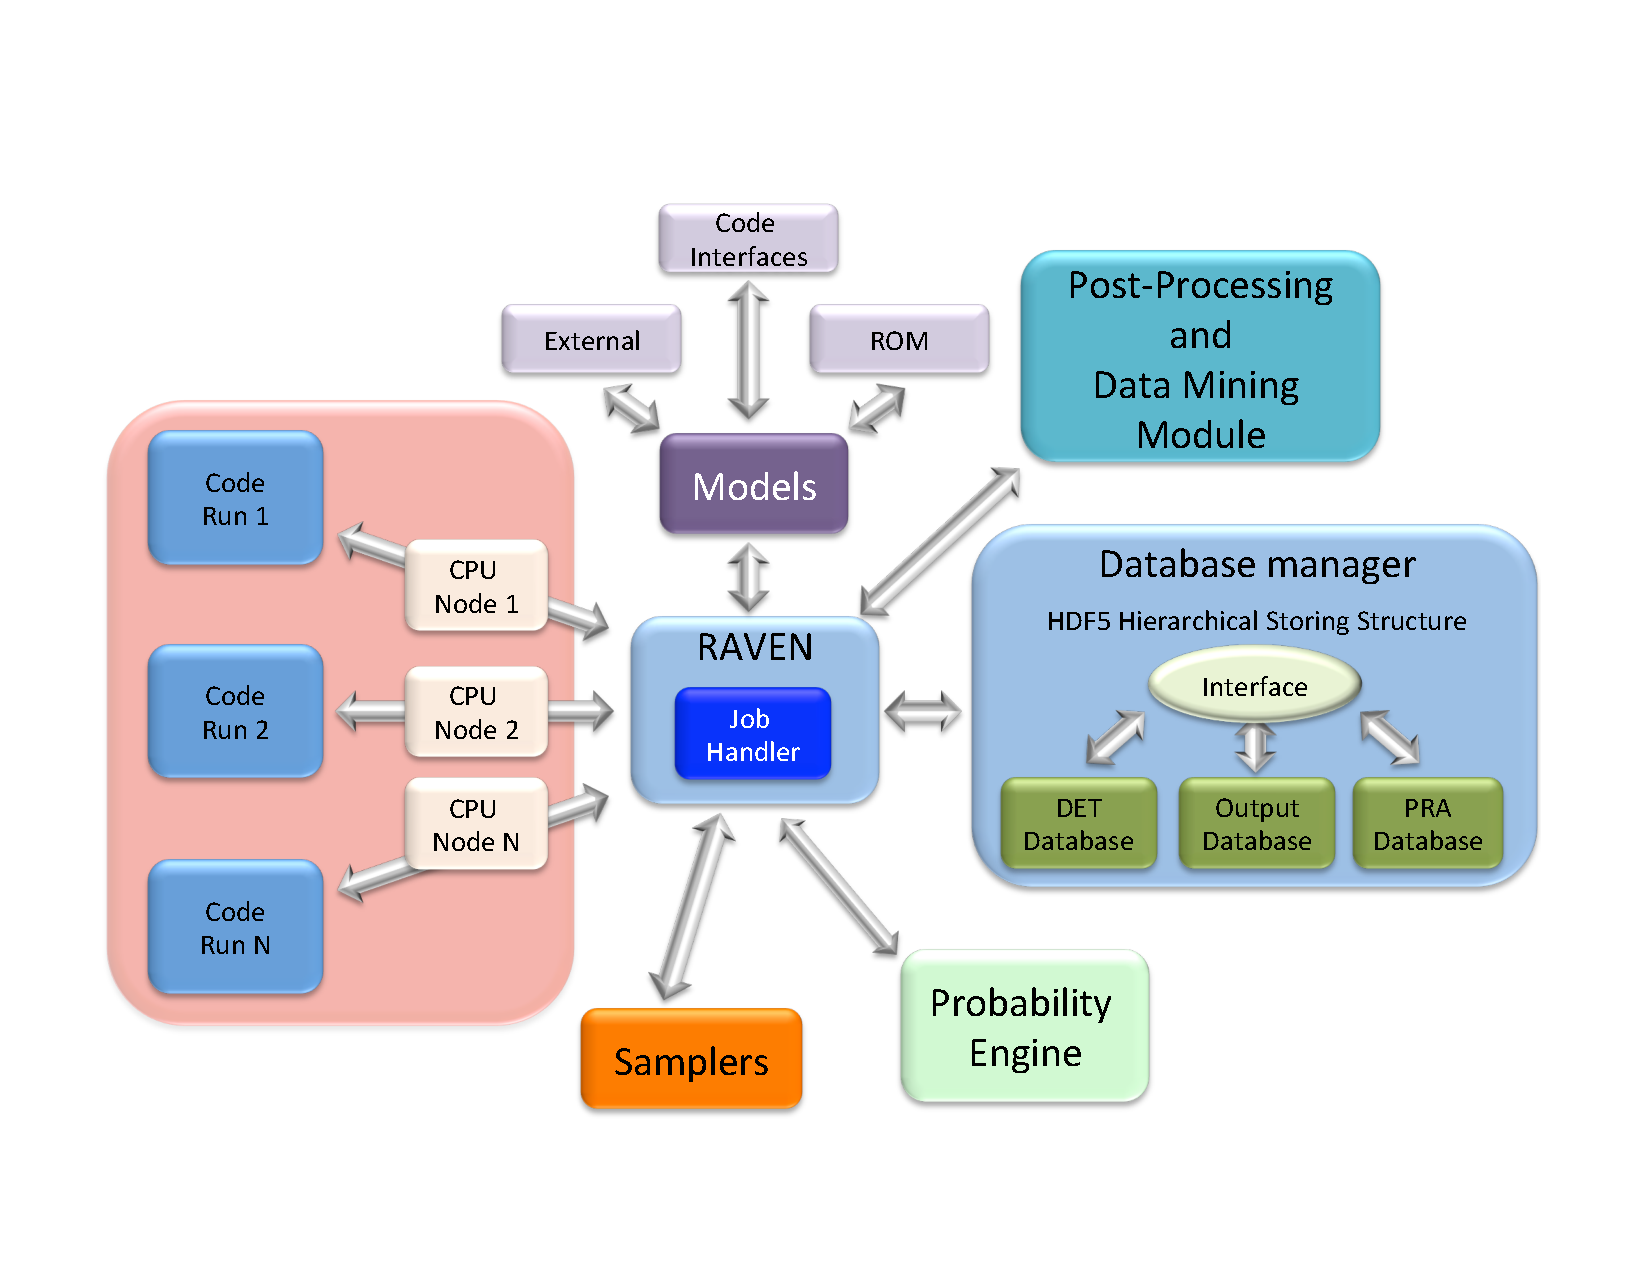
\includegraphics[scale=0.5]{raven.pdf}
    \caption{RAVEN}
    \label{fig:raven}
\end{figure}

\section{RISMC Approach to PRA}
\label{sec:rismc}

The RISMC approach~\cite{RISMC} employs both deterministic and stochastic methods 
in a single analysis framework (see Figure~\ref{fig:RISMCoverview}). In the deterministic method 
set we include:
\begin{itemize}
  \item Modeling of the thermal-hydraulic behavior of the plant~\cite{BWR_SBO_Mandelli,BWRanalysis}
  \item Modeling of external events such as flooding~\cite{mandelliPSA2015}
  \item Modeling of the operators’ responses to the accident scenario~\cite{HRA_BoringReport2014}
\end{itemize}

\begin{figure}
    \centering
    \centerline{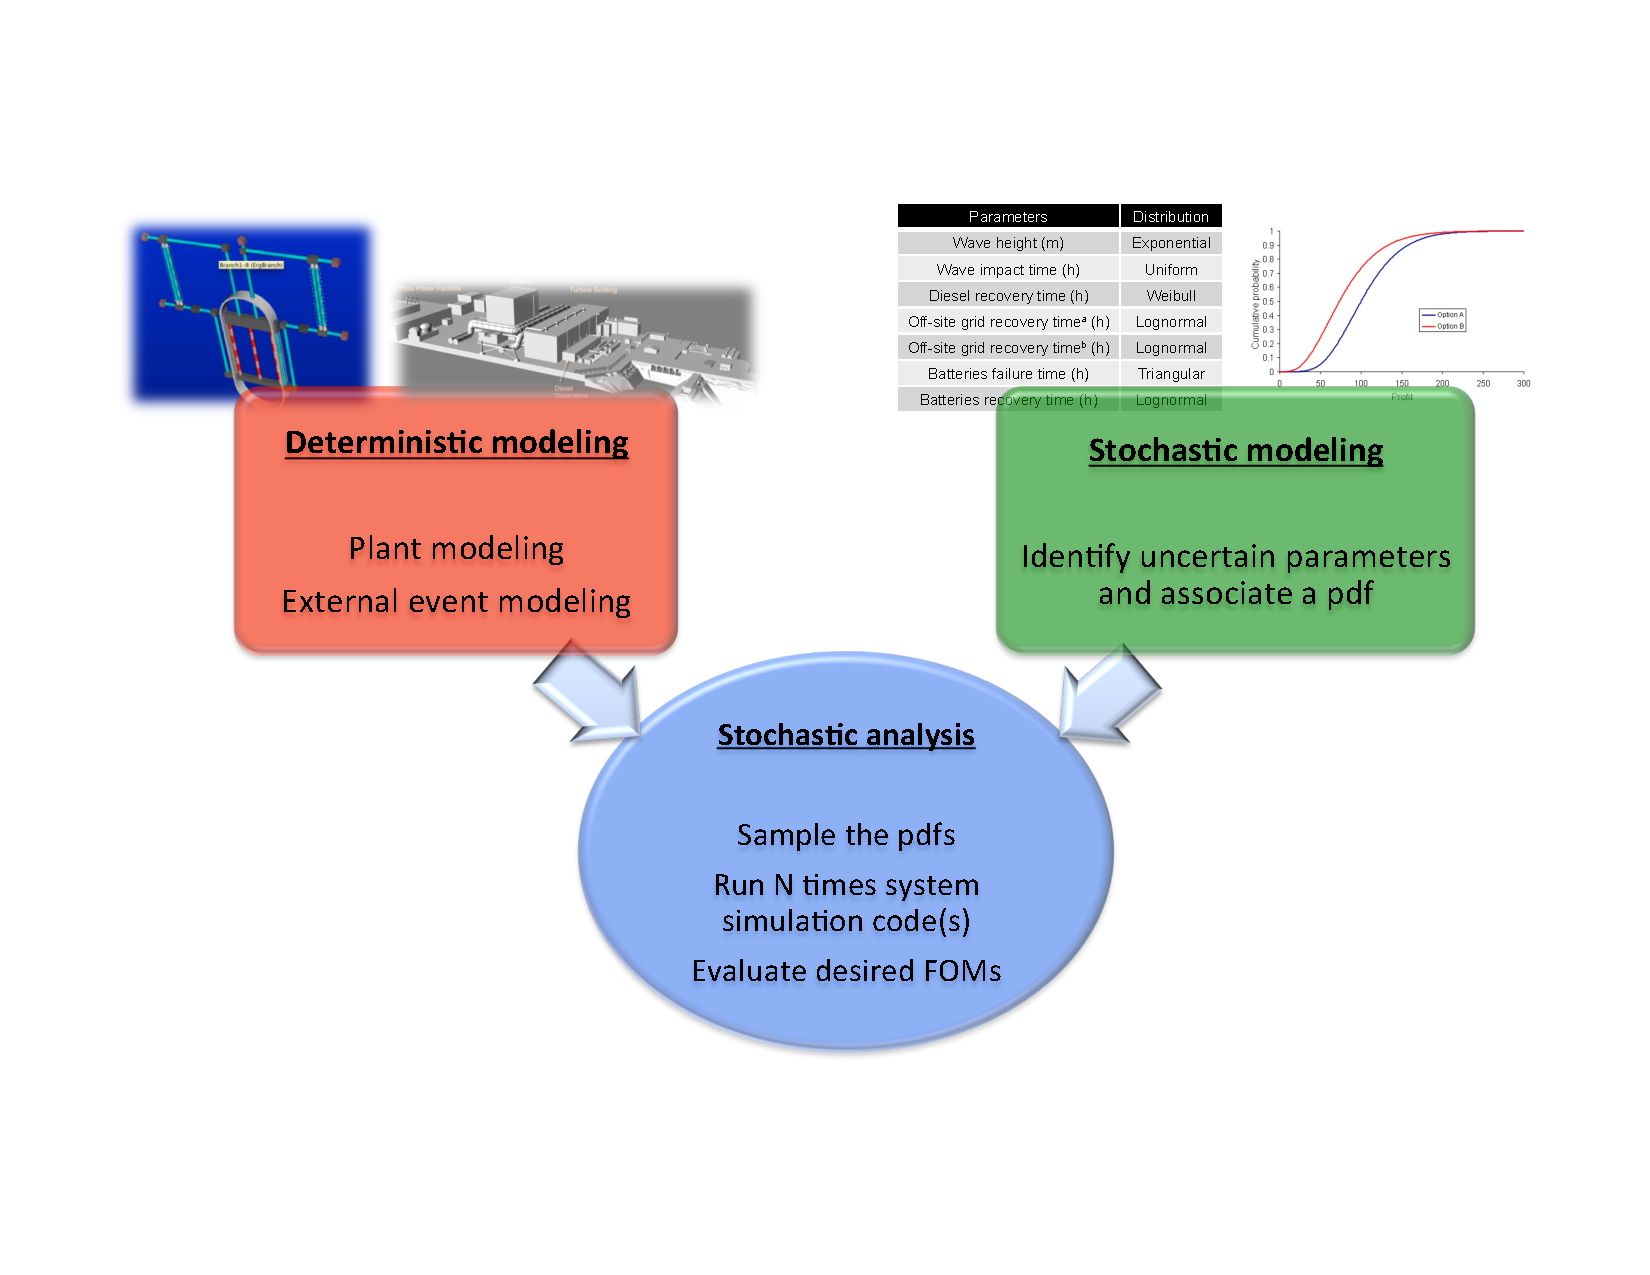
\includegraphics[scale=0.4]{RISMCoverview.pdf}}
    \caption{Overview of the RISMC approach}
    \label{fig:RISMCoverview}
\end{figure}

Note that deterministic modeling of the plant or external events can be performed by employing specific 
simulator codes but also surrogate models~\cite{ROM}, known as reduced order models (ROM). ROMs would 
be employed 
in order to decrease the high computational costs of employed codes. In addition, multi-fidelity codes 
can be employed to model the same system; the idea is to switch from low-fidelity to high-fidelity code 
when higher accuracy is needed (e.g., use low-fidelity codes for steady-state conditions and high-fidelity 
code for transient conditions)

In the stochastic modeling we include all stochastic parameters that are of interest in the PRA analysis 
such as uncertain parameters and stochastic failure of system/components.
As mentioned earlier, the RISMC approach heavily relies on multi-physics system simulator codes 
(e.g., RELAP5-3D~\cite{relap5}) coupled with stochastic analysis tools (e.g., RAVEN~\cite{raven}).  
From a PRA point of view, this type of simulation can be described by using two sets of variables:
\begin{itemize}
  \item $\boldsymbol c = \boldsymbol c(t)$ represents the status of components and systems of the simulator 
        (e.g., status of emergency core cooling system, AC system)
  \item $\boldsymbol \theta = \boldsymbol \theta (t)$ represents the temporal evolution of a simulated 
        accident scenario, i.e., $\boldsymbol \theta (t)$ represents a single simulation run. 
        Each element of $\boldsymbol \theta$ can be for example the values of temperature or pressure in 
        a specific node of the simulator nodalization.
\end{itemize}

From a mathematical point of view, a single simulator run can be represented as a single trajectory in the 
phase space. The evolution of such a trajectory in the phase space can be described as follows:
\begin{equation}
  \begin{cases}
    \dfrac{\partial \boldsymbol \theta }{\partial t}  = \boldsymbol \Xi (\boldsymbol \theta , \boldsymbol c, \boldsymbol s , t)   \\ \\ 
    \dfrac{\partial \boldsymbol c }{\partial t}  = \boldsymbol \Gamma (\boldsymbol \theta , \boldsymbol c, \boldsymbol s , t) 
  \end{cases}    
  \label{eq:trajectory}
\end{equation}
where:
\begin{itemize}
  \item $\boldsymbol \Xi$ is the actual simulator code that describes how θ evolves in time
  \item $\boldsymbol \Gamma$ is the operator which describes how c evolves in time , i.e., the status 
        of components and systems at each time step
  \item $\boldsymbol C$ is the set of stochastic parameters.
\end{itemize}

Starting from the system located in an initial state, $\boldsymbol \theta (t=0) = \boldsymbol \theta(0)$, 
and the set of stochastic parameters (which are generally generated through a stochastic sampling process), 
the simulator determine at each 
time step the temporal evolution of $\boldsymbol \theta (t)$. At the same time, the system control logic  
determines the status of the system and components $\boldsymbol c(t)$.
 
By using the RISMC approach, the PRA analysis is performed by~\cite{}:
\begin{enumerate}
  \item Associating a probabilistic distribution function (pdf) to the set of parameters 
        $\boldsymbol s$ (e.g., timing of events)
  \item Performing stochastic sampling of the pdfs defined in Step 1
  \item Performing a simulation run given $\boldsymbol s$ sampled in Step 2, i.e., solve the 
        system of equations~\ref{??}
  \item Repeating Steps 2 and 3 $M$ times and evaluating user defined stochastic parameters such 
        as core damage (CD) probability ($P_{CD}$).
\end{enumerate}

\section{RISMC Approach and Classical PRA}
\label{sec:analogy}

In order to better understand the results obtained in Section~\ref{sec:test} it is worth to illustrate 
a link between classical PRA and RISMC approach.
Let's consider a system that is composed by two components (i.e, A and B) in a series configuration where
each component has a failure probability (i.e., $p_A$ and $p_B$ respectively) as shown in Fig.~ref{}.

In a classical PRA framework such system can be modeled using a FT method that is composed by two basic events:
A failed and B failed.
System failure would be represented by a single ``AND'' gate that combine the two basic events as shown in 
Fig.~ref{}.

\begin{figure}
  \centering
  \begin{subfigure}{.5\textwidth}
    \centering
    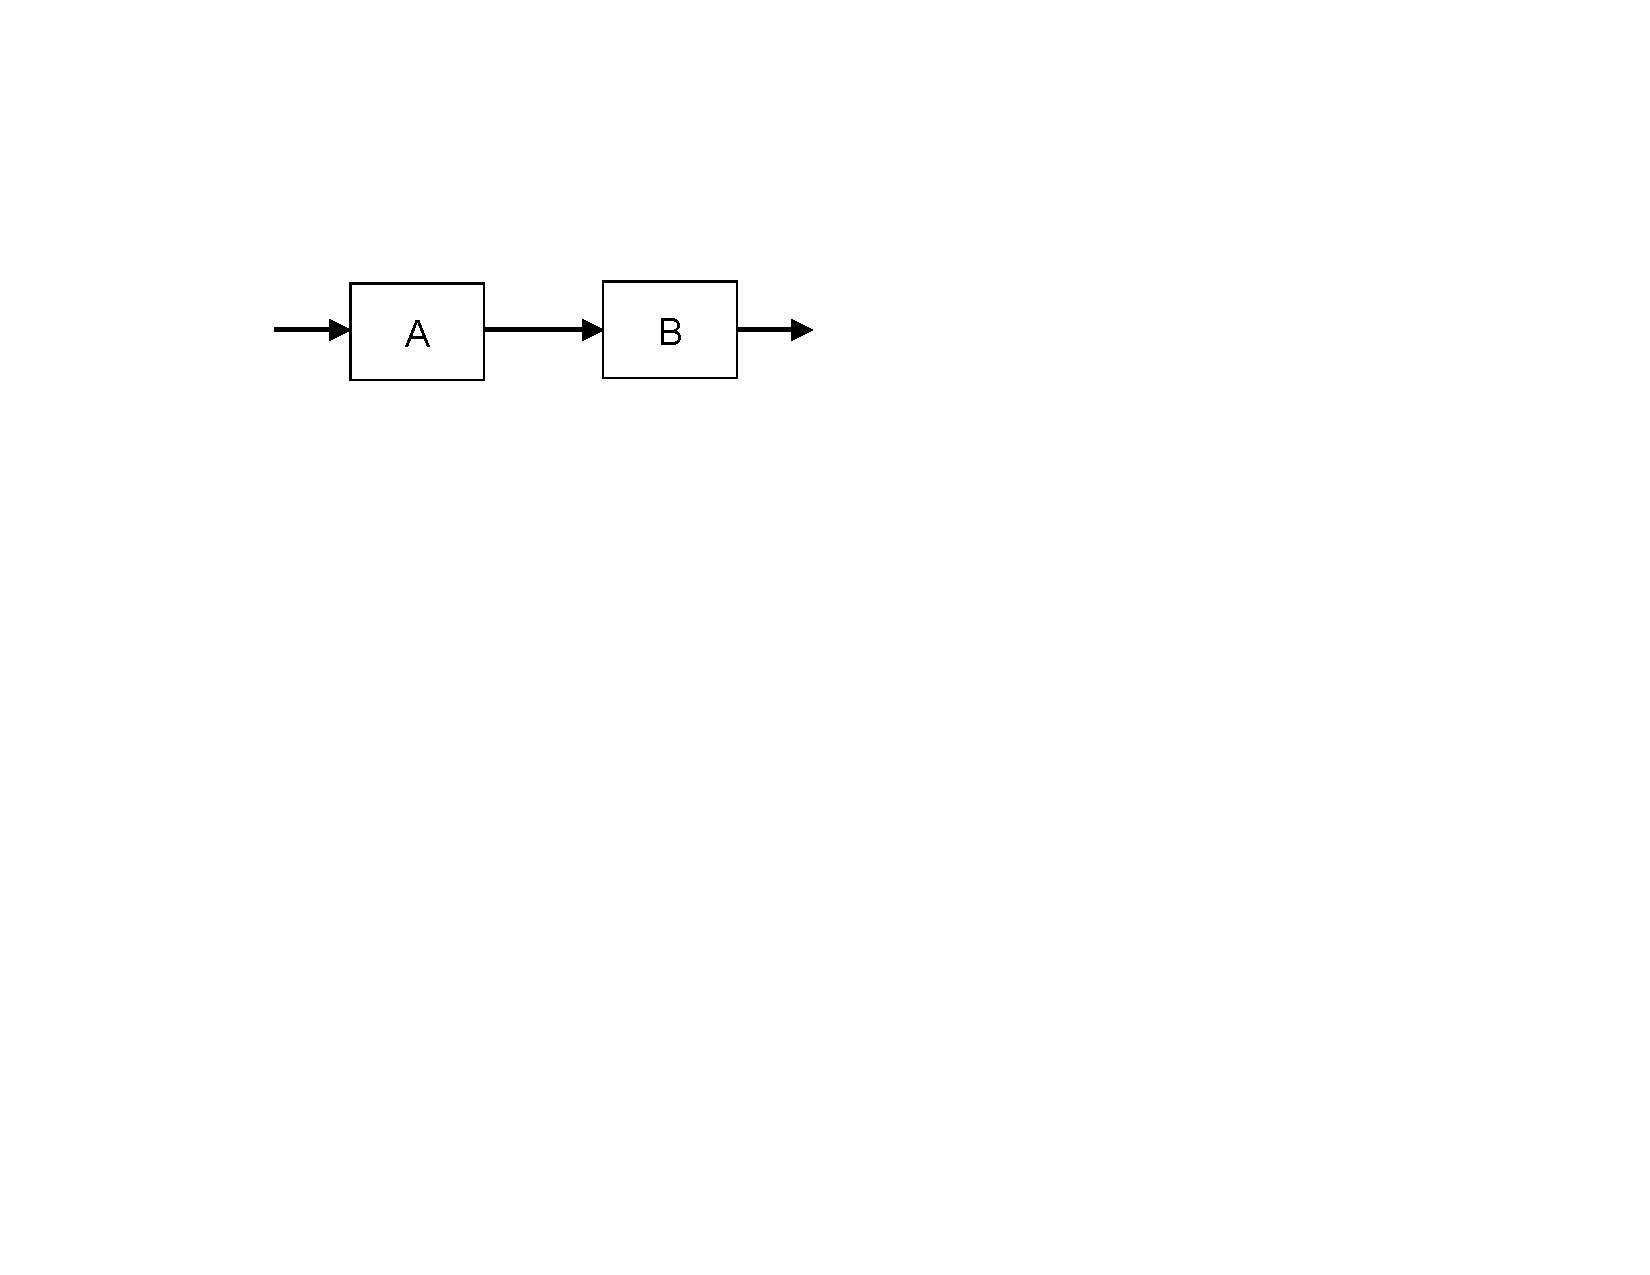
\includegraphics[scale=0.6]{ABsystem.pdf}
    \label{fig:sub1}
  \end{subfigure}%
  \begin{subfigure}{.5\textwidth}
    \centering
    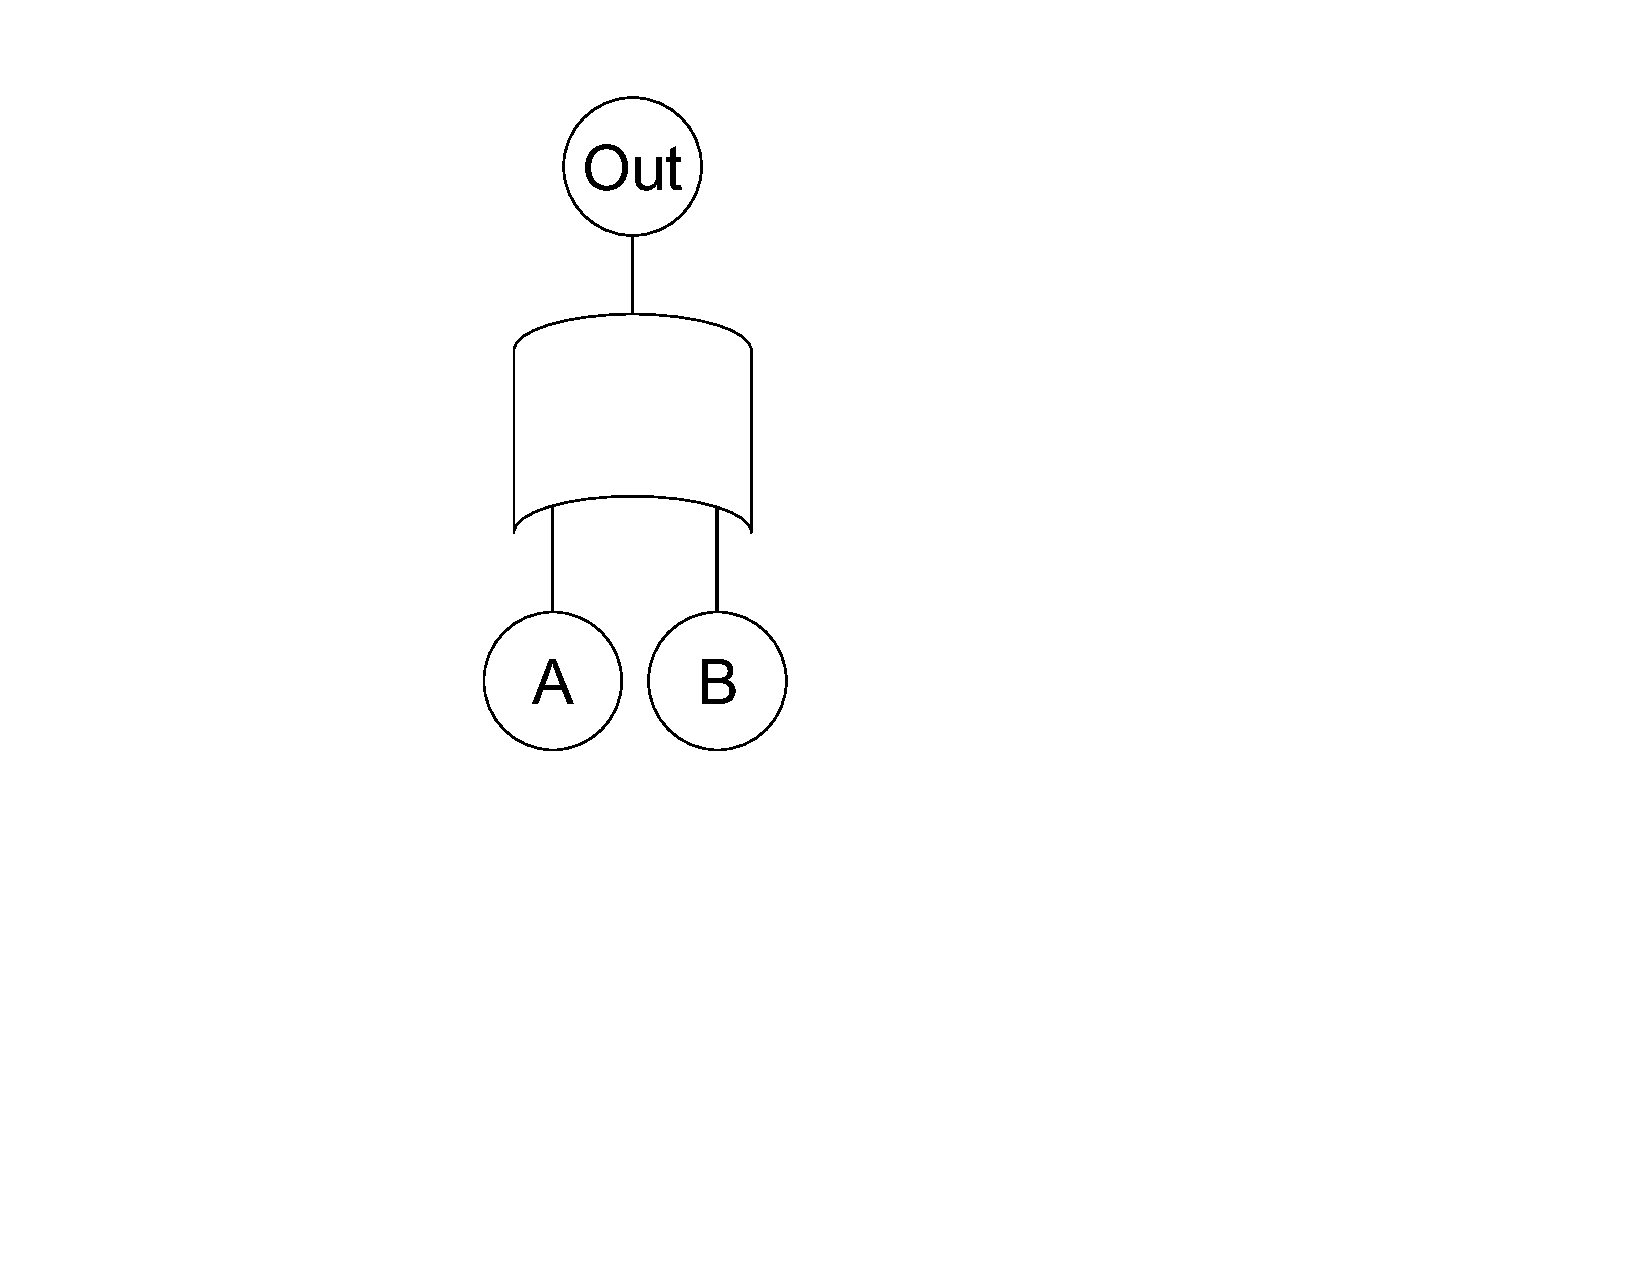
\includegraphics[scale=0.3]{andGate.pdf}
    \label{fig:sub2}
  \end{subfigure}
  \caption{Components A and B in a series configuration (left) and associated Fault-Tree (right).}
  \label{fig:chebyshev}
\end{figure}

\begin{figure}
    \centering
    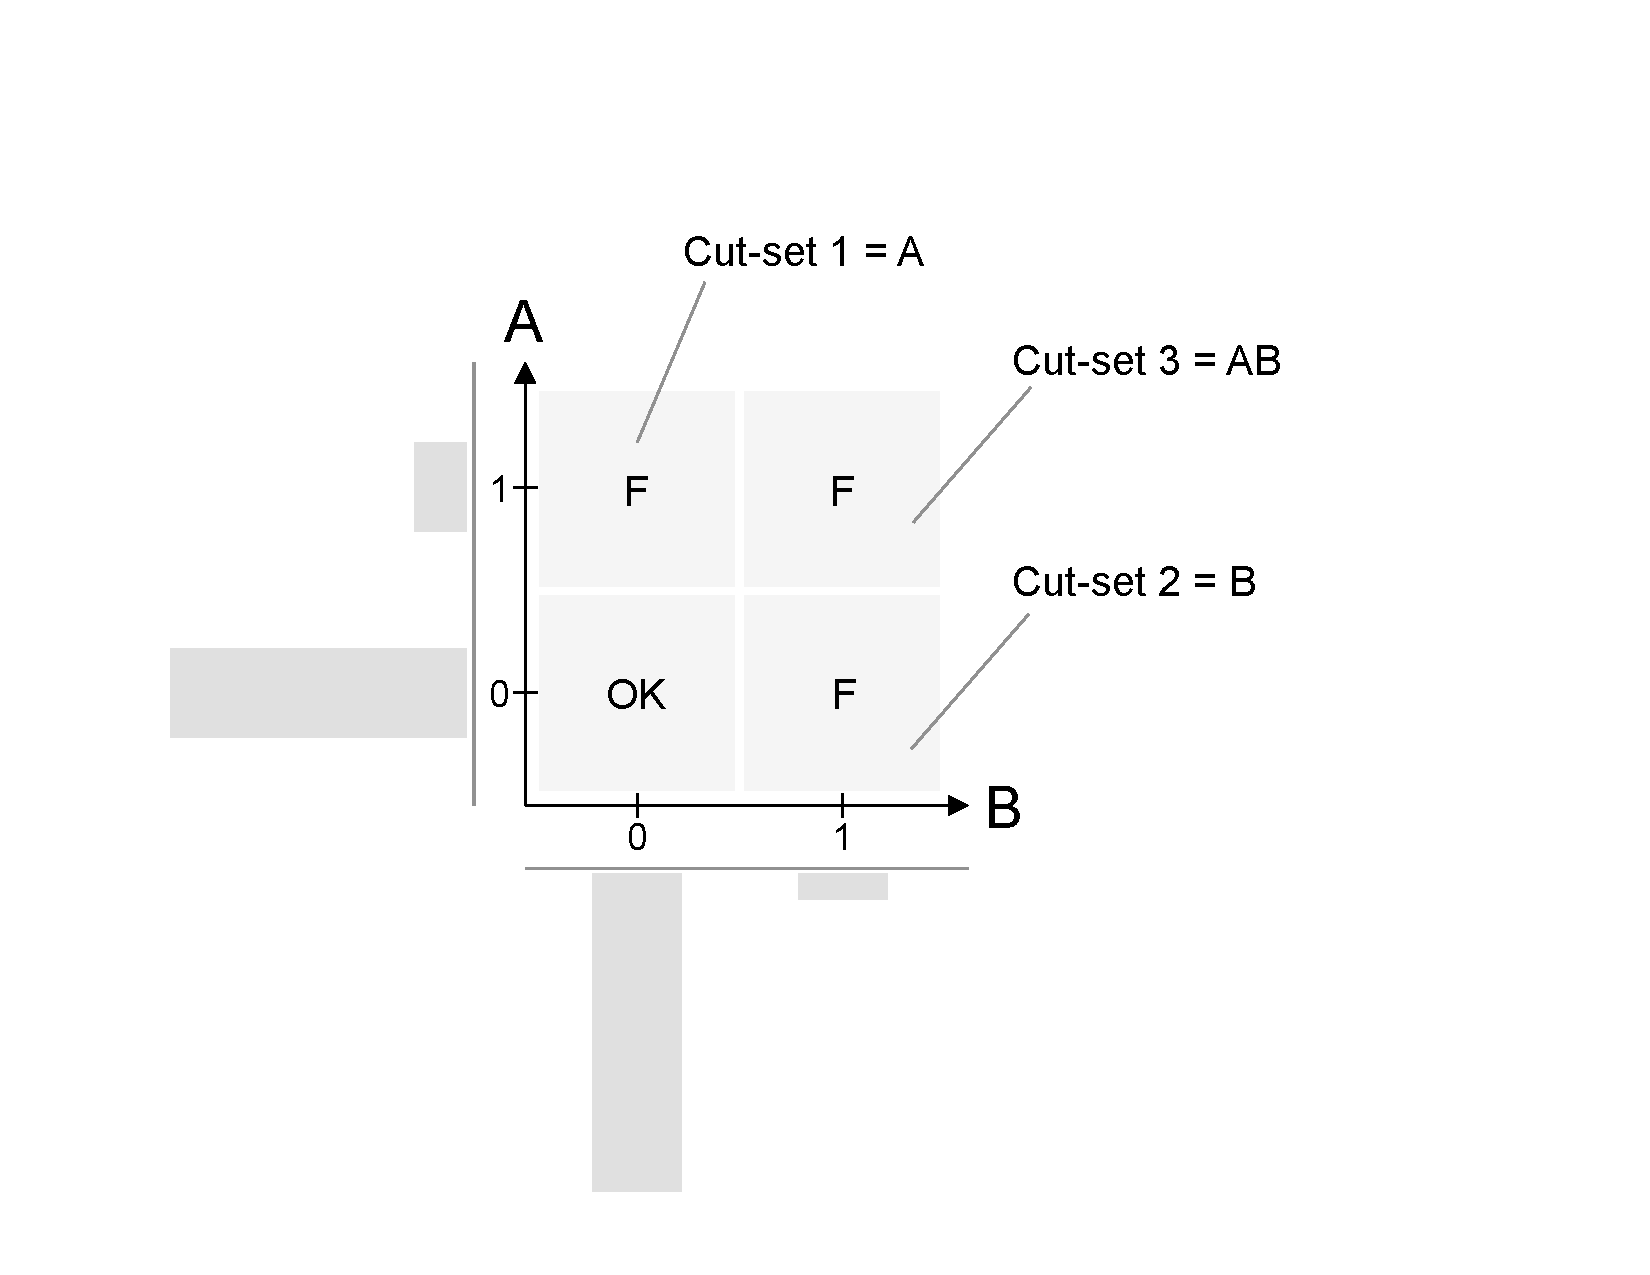
\includegraphics[scale=0.4]{2D.pdf}
    \caption{}
    \label{fig:2Danalogy}
\end{figure} 




\section{RAVEN}
\label{sec:raven}
 
The Risk Analysis and Virtual ENviroment 
(RAVEN\footnote{Official website: \url{https://raven.inl.gov},\\ 
GITHUB repository: \url{https://github.com/idaholab/raven}})
~\cite{RAVEN_PSAM_2014,alfonsiEsrel2014} 
is a flexible and multi-purpose uncertainty quantification, regression analysis, probabilistic
risk assessment, data analysis and model optimization framework. Depending on the tasks to be 
accomplished and on the probabilistic characterization of the problem, RAVEN perturbs 
(e.g., Monte-Carlo, latin hypercube, reliability surface search) the response of the system 
under consideration by altering its own parameters. The system is modeled by third party software 
(e.g., RELAP5-3D~\cite{relap5}, MELCOR~\cite{Melcor}) and accessible to RAVEN either directly 
(software coupling) or indirectly (via input/output files). 
The data generated by the sampling process is analyzed using 
classical statistical and more advanced data mining approaches. RAVEN also manages the parallel dispatching 
(i.e. both on desktop/workstation and large High Performance Computing machines) of the software 
representing the physical model. RAVEN heavily relies on artificial intelligence algorithms to construct 
surrogate models of complex physical systems in order to perform uncertainty quantification, reliability 
analysis (limit state surface) and parametric studies.

By statistical analysis we include:
\begin{itemize}
  \item Sampling of codes, either stochastic, e.g., Monte-Carlo~\cite{DynamicReliabilityMonteCarlo} 
        and Latin Hypercube Sampling (LHS)~\cite{LHShelton}, deterministic (e.g., grid and
        Dynamic Event Tree (DET)~\cite{AMENDOLAdylam,cojazziDylam}) or 
        adaptive~\cite{ANS_S_2014_raven_LS,mandelliSVMANS}
  \item Generation of ROMs~\cite{ROM_Khalik}, also known as Surrogate models
  \item Post-processing of the sampled data and generation of statistical parameters (e.g., mean, 
        variance, covariance matrix).
\end{itemize}

Figure~\ref{fig:ravenScheme} shows a general overview of the elements that comprise the RAVEN 
statistical framework:

\begin{itemize}
  \item Model: it represents the pipeline between input and output space. It comprises both codes 
        (e.g., RELAP5-3D~\cite{relap5}) and also ROMs 
  \item Sampler: it is the driver for any specific sampling strategy, e.g., Monte-Carlo, LHS, 
        DET~\cite{ANS2014_adaptDET,PSA2013_Raven})
  \item Database: the data storing entity
  \item Post-processing module: the module that performs statistical analyses and visualizes results.
\end{itemize}

\begin{figure}
    \centering
    \centerline{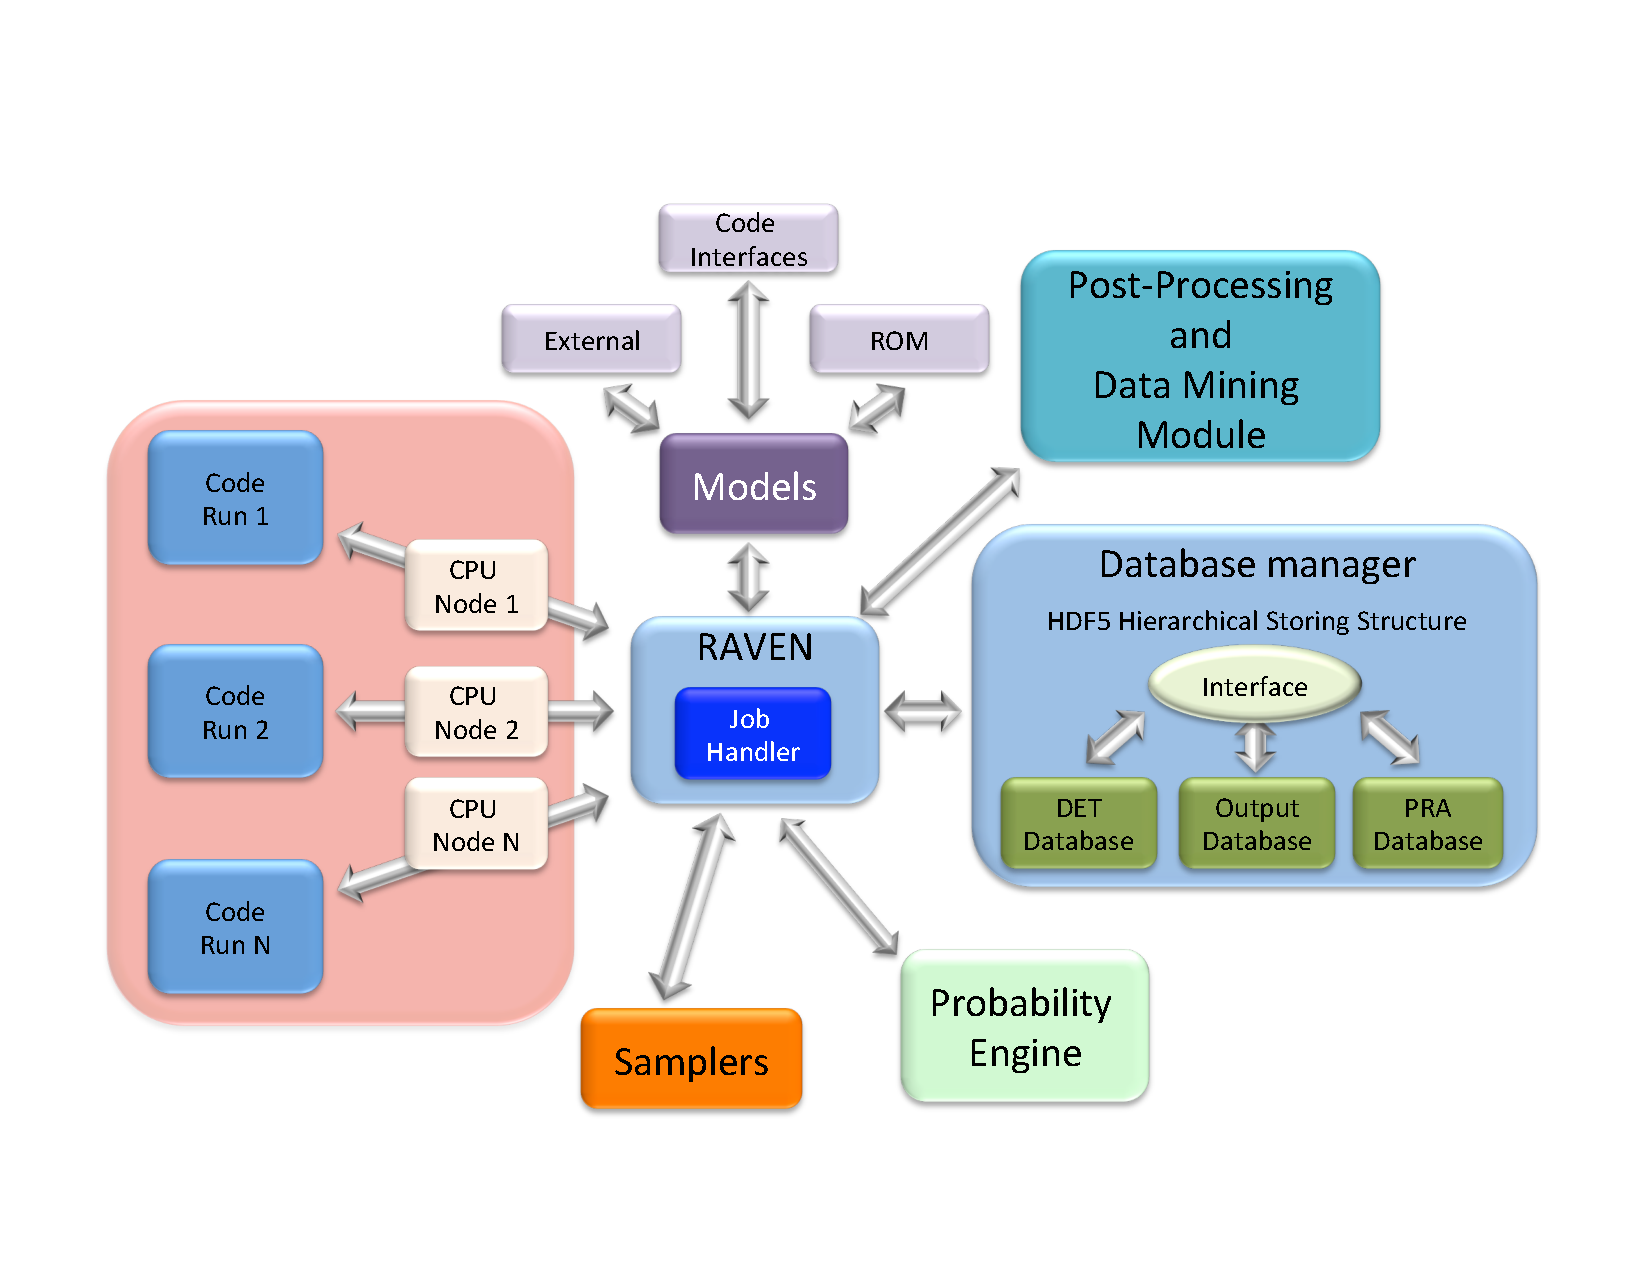
\includegraphics[scale=0.4]{raven.pdf}} 
    \caption{Overview of RAVEN statistical framework components}
    \label{fig:ravenScheme}
\end{figure}

\subsection{Ensemble-Model Capabilities}

In several cases multiple models need to interface with each other since the initial 
conditions of some are dependent on the outcomes of others. In order to face this problem 
in the RAVEN framework, a new model category (e.g., class), named EnsambleModel, was 
implemented~\cite{alfonsiEnsemble}. This class is able to assemble multiple models of 
other categories (i.e. Code, External Model, ROM), identifying the input/output connections, 
and, consequentially the order of execution and which sub-models can be executed in parallel. 
 
\begin{figure}
    \centering
    \centerline{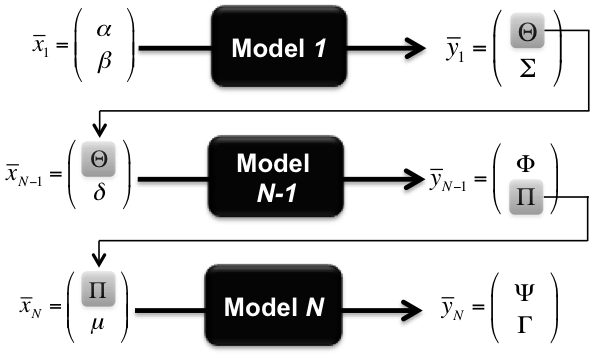
\includegraphics[scale=0.7]{LinearEnsemble.png}} 
    \caption{Example of an EnsembleModel constituted by 3 sequential sub-models.}
    \label{fig:exampleEnsembleModel}
\end{figure}
 
Figure~\ref{fig:exampleEnsembleModel} reports an example of an EnsembleModel that is constituted by 
3 sub-models (ROMs, Codes, or External Models). As it can be noticed:

\begin{itemize}
  \item The Model 2 is connected with the Model 1 through the variable $\Theta$ (Model 1 output and Model 2 input);
  \item The Model 3 is connected with the Model 2 through the variable $\Pi$ (Model 2 output and Model 3 input);
\end{itemize}

In this case, the EnsembleModel is going to drive the execution of all the sub-models in a serial sequence, 
since each model (except the Model 1) is dependent on one of the outcomes of previously executed.
In several cases, the input of a model depends on the output of another model whose input is the output 
of the initial model. In this situation, the system of equation is non-linear and an iterative solution 
procedure needs to be employed. The EnsembleModel entity in RAVEN is able to detect the non-linearity of 
the sub-models’ assembling and activate the non-linear solver: an iterative scheme. 

Figure~\ref{fig:exampleEnsembleModelNonLinear} shows an example 
of when the EnsembleModel entity activates the iteration scheme, which ends when the residue norm 
(between an iteration and the other) falls below a certain input-defined tolerance.

 \begin{figure}
    \centering
    \centerline{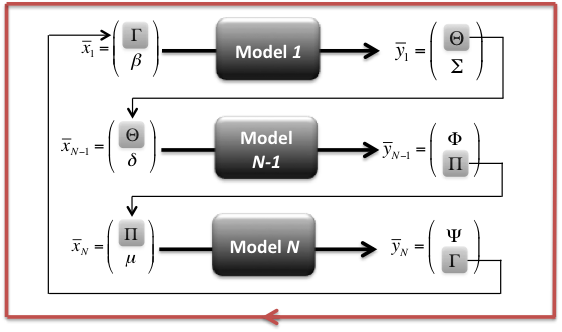
\includegraphics[scale=0.8]{NonLinearEnsemble.png}} 
    \caption{EnsembleModel resolving in a non-linear system of equations – Numerical iterations.}
    \label{fig:exampleEnsembleModelNonLinear}
\end{figure}

In RAVEN all the models’ outputs (e.g., whatever code output, etc.) are collected in internal containers 
(named DataObjects) that are aimed to store time-series and input/output data relations in a standardized 
fashion; in this way, the communication of the output information among different entities (i.e., Models) 
can be completely agnostic with respect to the particular type of output generated by a 
model.

 
\section{Multi-Unit Modeling}
\label{sec:multiUnitModeling}

From a mathematical point of view, a single simulator run can be represented 
as a single trajectory in the phase space. The evolution of such a trajectory 
in the phase space as function of time $t$ can be described as follows:
\begin{equation}
    \frac{\partial \boldsymbol \theta }{\partial t}  = \boldsymbol \Xi (\boldsymbol \theta , \boldsymbol p, \boldsymbol s , t) 
    \label{eq:trajectory}
\end{equation}
where:
\begin{itemize}
  \item $\boldsymbol \theta = \boldsymbol \theta(t)$ represents the temporal 
        evolution of a simulated accident scenario, i.e., $\boldsymbol \theta(t)$ can 
        represent temperature inside the reactor core, the pressure level inside a containment
        building, the radionuclide concentration at a specific point outside the plant, etc.
  \item $\boldsymbol \Xi$ is the actual simulator code that describes how $\boldsymbol \theta$ 
        evolves in time
  \item $\boldsymbol s = \boldsymbol s(t,\boldsymbol p)$ represents the status of components 
        and systems of the model (e.g., status of emergency core cooling system, AC system)
\end{itemize}

By using the RISMC approach, if Monte-Carlo sampling is chosen, the PRA analysis is performed 
by~\cite{BWR_SBO_Mandelli}:
\begin{enumerate}
  \item Associating a probabilistic distribution function (pdf) to the set of uncertain 
        parameters $\boldsymbol p$ (e.g., timing of events)
  \item Performing stochastic sampling of the pdfs defined in Step 1
  \item Performing a simulation run given $\boldsymbol p$ sampled in Step 2, i.e., solve Eq.~\ref{eq:trajectory}
  \item Repeating Steps 2 and 3 $M$ times and evaluating user defined stochastic parameters such as 
        Core Damage (CD) probability $P_{CD}$ as
        \begin{equation}
            P_{CD} = \frac{M_{CD}}{M} 
            \label{eq:CDprobability}
        \end{equation}
        where $M_{CD}$ is the number of simulations that lead to CD. 
\end{enumerate}

In a multi-unit type of scenario, the dynamic behaviour of each unit is not independent but it can actually 
interact with the other units. Example of interactions are: electrical cross-ties and shared plant 
resources such as portable AC generators

Since Equation~\ref{eq:trajectory} refers to a single unit plant site, if multiple units are considered 
then it is needed to track the temporal evolution of each unit,i.e., multiple $\theta$ needs to be evaluated 
(one for each unit). 
Assuming that a three-unit plant is considered, Eq.~\ref{eq:trajectory} now becomes as follows:

\begin{equation}
  \begin{matrix}
     \begin{dcases*}
       \frac{\partial \boldsymbol{\theta}_1}{\partial t}  = \boldsymbol{\Xi}_1 (\boldsymbol{\theta}_1 , \boldsymbol p, \boldsymbol{s}_1 , \boldsymbol{s}_2 , \boldsymbol{s}_3, t)  \\     
       \frac{\partial \boldsymbol{\theta}_2}{\partial t}  = \boldsymbol{\Xi}_2 (\boldsymbol{\theta}_2 , \boldsymbol p, \boldsymbol{s}_1 , \boldsymbol{s}_2 , \boldsymbol{s}_3, t)  \\   
       \frac{\partial \boldsymbol{\theta}_3}{\partial t}  = \boldsymbol{\Xi}_3 (\boldsymbol{\theta}_3 , \boldsymbol p, \boldsymbol{s}_1 , \boldsymbol{s}_2 , \boldsymbol{s}_3, t)  \\       
     \end{dcases*}
  \end{matrix}
  \label{eq:MU_looseCoupled}
\end{equation}

Note that now the vector $s_i (i=1,\ldots,3)$ of each unit is shared among other units. This feature 
captures shared resources and possible system cross-ties among units.
In addition, intra-unit interactions (such as a sub-set of human actions in a unit) may be driven 
by the actual status of other unit (e.g., thermo-hydraulic limit and operational boundaries). 
Again, these actions may have cascade effects on the other units. This is particularly relevant 
for severe accident scenarios. Thus, now Eq.~\ref{eq:MU_looseCoupled} becomes:

\begin{equation}
  \begin{matrix}
     \begin{dcases*}
       \frac{\partial \boldsymbol{\theta}_1}{\partial t}  = \boldsymbol{\Xi}_1 (\boldsymbol{\theta}_1 , \boldsymbol{\theta}_2, \boldsymbol{\theta}_3 , \boldsymbol p, \boldsymbol{s}_1 ,
       \boldsymbol{s}_2 , \boldsymbol{s}_3, t)  \\
       \frac{\partial \boldsymbol{\theta}_2}{\partial t}  = \boldsymbol{\Xi}_2 (\boldsymbol{\theta}_1 , \boldsymbol{\theta}_2, \boldsymbol{\theta}_3 , \boldsymbol p, \boldsymbol{s}_1 ,
       \boldsymbol{s}_2 , \boldsymbol{s}_3, t)  \\
       \frac{\partial \boldsymbol{\theta}_3}{\partial t}  = \boldsymbol{\Xi}_3 (\boldsymbol{\theta}_1 , \boldsymbol{\theta}_2, \boldsymbol{\theta}_3 , \boldsymbol p, \boldsymbol{s}_1 ,
       \boldsymbol{s}_2 , \boldsymbol{s}_3, t)  \\
     \end{dcases*}
  \end{matrix}
  \label{eq:MU_tightCoupled}
\end{equation}

From a modeling point of view, solving Eq.~\ref{eq:MU_looseCoupled} or Eq.~\ref{eq:MU_tightCoupled} poses 
different challenges. Equation~\ref{eq:MU_looseCoupled} can in fact be solved by:
\begin{itemize}
  \item Sampling the set of uncertain parameters $\boldsymbol p$
  \item Determining the temporal profile of $\boldsymbol{s}_1$, $\boldsymbol{s}_2$, $\boldsymbol{s}_3$
  \item Run the simulator for each unit independently given $\boldsymbol p$, $\boldsymbol{s}_1$, $\boldsymbol{s}_2$, $\boldsymbol{s}_3$
\end{itemize}

On the other side, solving Eq.~\ref{eq:MU_tightCoupled} requires a system simulator that allows 
running the simulation of each unit simultaneously and sharing the variables
$\boldsymbol{\theta}_1$, $\boldsymbol{\theta}_2$, $\boldsymbol{\theta}_3$ among them.
This paper will focus on multi-unit case that can be described by Eq.~\ref{eq:MU_looseCoupled}. 




\section{Test Case}
\label{sec:testCase}

\subsection{Plant Description}
For the scope of this paper we have chosen a 3-unit plant as shown in Figure 2. 
In more detail, the system we have considered is the following (see Table 1):
\begin{itemize}
  \item Unit 1: 1 PWR (see Figure 3) at full power (100 \%) and it own Spent Fuel Pool (SFP)
  \item Unit 2: 1 PWR in mid-loop operation (i.e., shut-doen mode) and it own SFP. 
                The mid-loop status is characterized by a primary coolant system drained to the 
                hot leg centerline and the existence of openings which a further reduction of 
                the mass inventory poses a serious risk, due to boil off and possible entrainment 
                or spill over of liquid
  \item Unit 3: 1 PWR at full power (108 \%) that restarted a few weeks earlier and its own SFP 
                with a higher heat load since it contains used fuel recently moved from the reactor.
\end{itemize}

In addition, special attention has been given to the design of the electrical and hydraulic systems (see Figure 5):
\begin{itemize}
  \item The plant electrical system is shown in Figure 4. Two electrical switchyards can provide 
        electrical power to all units. All units have a set of Emergency Diesel Generators (EDGs) 
        and, in addition, a swing EDG (i.e., EDGS) can be employed to provide an alternate AC power to either
        Unit 1 or Unit 2. Note also that the 6.6 KV emergengy buses of Unit 1 and Unit 2 can be cross-tied.
  \item The auxiliary feedwtaer (AF) system of Unit 1 and Unit 3 can be cross-tied. Thus cooling to the 
        secondary side can be provided from one unit to the other one.
  \item The Condensate Storage Tanks (CSTs) of Units 2 and Unit 3 can be cross-tied. Thus the water source 
        for the secondary side of either unit can be used as water source for the other one.
\end{itemize}

Plant recovery crew is a shared resource within the plant. As part of the accident secnario, the recovery 
crew can perform AC power and safety injection using mobile equipment located within each unit.


\subsection{Initiaiting Event}

The considered accident scenario is a seisimc event which causes the following events:
\begin{itemize}
  \item Both swityards are disabled
  \item All EDGs are disabled except EDGS which is initially aligned to Unit 2
  \item CST of Unit 2 has lost 80\% of its capacity 
  \item CST of Unit 3 is completely lost
  \item The seisimic event might also rupture the SFPs. Thus a leak might be present during the accident scenario
\end{itemize}

The proposed accident scenario resembles a Station Black Out  (SBO) event at the plant level except for the 
fact that the EDGS is the only source of AC power available and it can be directed toward either Unit 1 or Unit 2.

\section{RISMC approach to multi-unit modeling}
\label{sec:RISMC_MU_modeling}



\subsection{RAVEN Ensemble-Model Capabilities}
[ANDREA]

\subsection{System Models}
[CARLO]
\subsubsection{PWR1 and PWR3}

\subsubsection{PWR2}

\subsubsection{SFPs}

\subsubsection{Human models}
[RON]

\subsection{Plant Model}

\section{toolkit}
\label{sec:toolkit}
\section{toolkit}
\label{sec:toolkit}
\section{Methods of Data Analysis}
\label{sec:plantAnalysisResults}

Historically the concept of CD probability has been typically 
associated to a single unit. At a plant level, a separate value of CD 
probability can be associated to all PWRs and SFPs. However, note that there 
is a high correlation among the six models of the plant site (PWRs and SFPs). 
Thus, a high correlation among CD probabilities of the six models is also expected.

Instead of defining a single CD probability value for each PWR and SFP 
we define a probability value to a Plant Damage State (PDS) variable. This 
variable is a $6$-dimensional vector where each vector element describes the 
status of a plant model. For the scope of this paper we allow two possible 
values to each element of the vector: OK or CD. Hence $2^6=64$ possible 
combinations are allowed.

In order to analyze the data generated by RAVEN we have selected a three steps 
approach:
\begin{enumerate}
  \item Group simulation runs based on their own PDS  
  \item Evaluate probability associated to each PDS and rank PDSs based on 
        their probability values.
  \item Identify communalities that characterize each PDS
\end{enumerate}

In order to perform such analysis, two post-processors were developed in RAVEN in 
addition to the ones already developed within RAVEN itself.
Thus the process of data generation, reduced order modeling and data analysis 
have been fully completed using the RAVEN code.
\section{toolkit}
\label{sec:toolkit}
\section{Conclusions}
\label{sec:conclusions}
In this paper, a newly developed capability of the RAVEN code has been shown. Through the Ensemble-Model entity, RAVEN is able to combine multiple models (i.e. Simulation Codes, Reduced Order Models, etc.), constructing a pipe network in order to transfer information among them. The addition of the Picard’s iteration scheme lets the user solving combinations of models that resolve in non-linear systems. 
The paper shows the early results for implementation of an ensemble approach for the coupling of surrogate models representing a multi-physics problem. While this is an initial implementation, the developed structure seems to support current needs and will be eventually extended in the future in order to couple codes whose input/output space is represented by high-density fields (e.g. temperature profiles in each nodal kinetic zones, etc.). This capability builds a complex system representation, even when the original models were not coupled, but just coupled their surrogate. Two applications are relevant for reliability analysis: (1) the possibility to build surrogate representation of a complex system, starting from libraries of surrogate models for each component, and (2) software implementation present during the first stage of surrogate model coupling when responses are high-density fields. 
The Ensemble-Model capability in RAVEN is currently used to couple a fuel performance code (Bison) and the T-H system code RELAP5 in order to analyze LOCA scenarios.ion.


\section*{References}

\bibliography{main}

\end{document}